\section{Uncertainty budget}\label{ch:Uncertainty}
Measuring the pion cross section  in LArIAT translates into counting how many pion impinged on a slab of argon at a given energy and how many of those pions interacted at said energy. So, the key questions here are:
\begin{itemize}
\item[]a) how well do we know that the $\pi/\mu/e$ candidate is a pion? Beam line contamination
\item[]b) how well do we know the kinetic energy at each point of the tracking? %(Incident Kinetic Energy bins)
\item[]c) how well do we know when the tracking stops? %(Interacting Kinetic Energy bin)
\end{itemize}


\section{Handling Beamline Contamination}


\section{Energy Studies}

A study we did was to look at the difference between DATA/MC in the dE/dX and energy deposited. We basically found there is very little difference between the two and we try to quantify how much the difference is.

%%%%%%%%%%%%%%%%%%%%%%%%%%%%%%%%%%%%%%%%%%%%%%%
\subsection{dE/dX}
%%%%%%%%%%%%%%%%%%%%%%%%%%%%%%%%%%%%%%%%%%%%%%%
Figure \ref{fig:dEdXLinearScale} shows the output of the fit of the Pion MC and the 60 Amp data. The MC is normalized to the data and both are fit to a Landau function. \footnote{The entries at dE/dX = 0 come from an uninitialized variable and can/should be taken out of these plots}

\begin{figure}[htb]
\centering
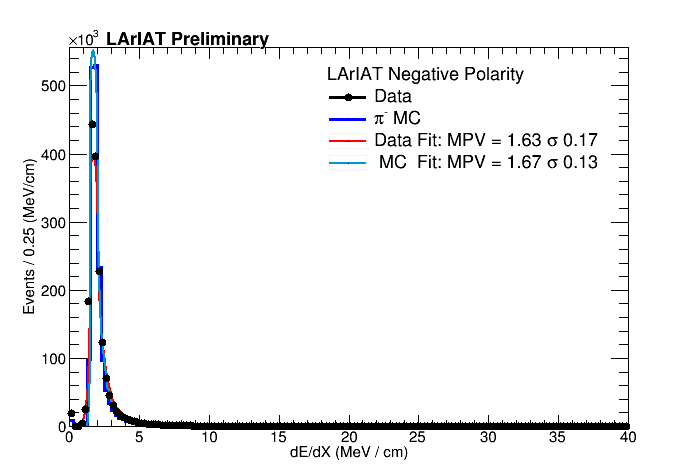
\includegraphics[width=0.48\textwidth]{Studies/Figures/dEdX_Fit_v1.png}
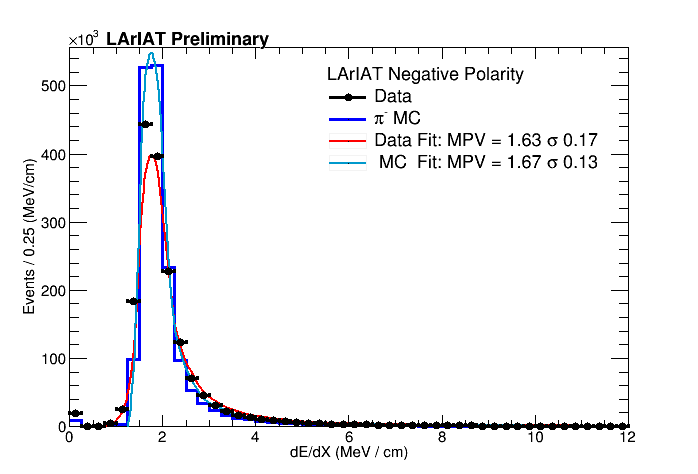
\includegraphics[width=0.48\textwidth]{Studies/Figures/dEdX_Fit_v4.png}
\caption[]{ dE/dX for 60Amp data and data driven pion MC, both fit with a Landau  } \label{fig:dEdXLinearScale}
\end{figure}

The difference between the two MPV's, is 2.4\% between the data and the MC.

Figure \ref{fig:dEdXLinearStacked} shows the stacked version of the dE/dX with the backgrounds stacked. The backgrounds are given in the ratio of 68.8\% pion, 4.6\% muon, and 26.6\% electron. Once they are taken in these ratios, the sum of the MC is normalized to the sum of the data.

\begin{figure}[htb]
\centering
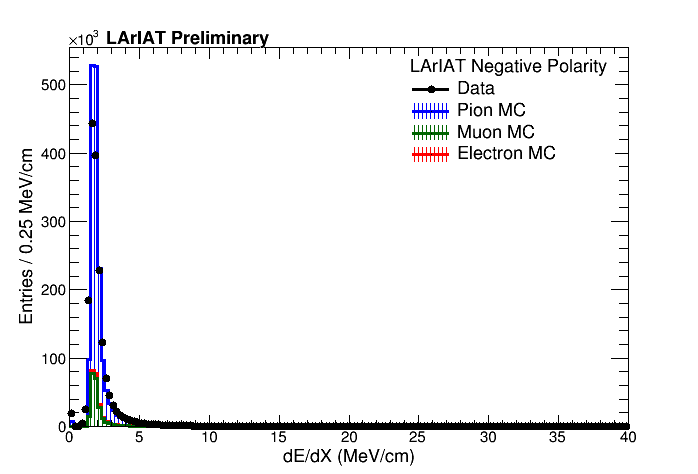
\includegraphics[width=0.48\textwidth]{Studies/Figures/dEdX_stacked_v1.png}
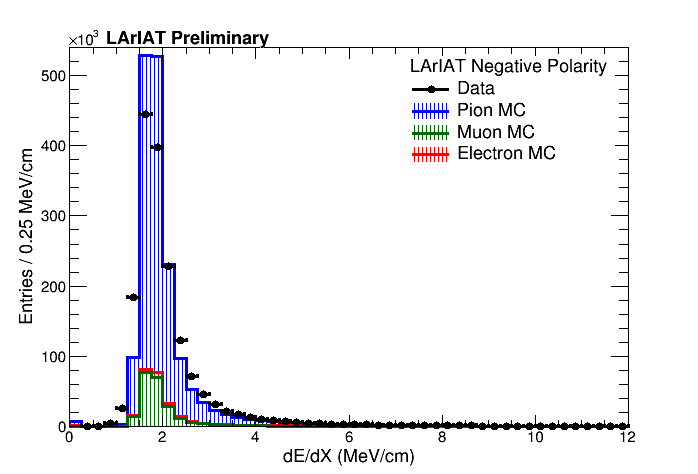
\includegraphics[width=0.48\textwidth]{Studies/Figures/dEdX_stacked_v4.png}
\caption[]{ Stacked versions of the dE/dX with the data and electron/muon/pion MC.  } \label{fig:dEdXLinearStacked}
\end{figure}

For completeness, the log scale versions of are shown in Figure \ref{fig:dEdXLogScale}.

\begin{figure}[htb]
\centering
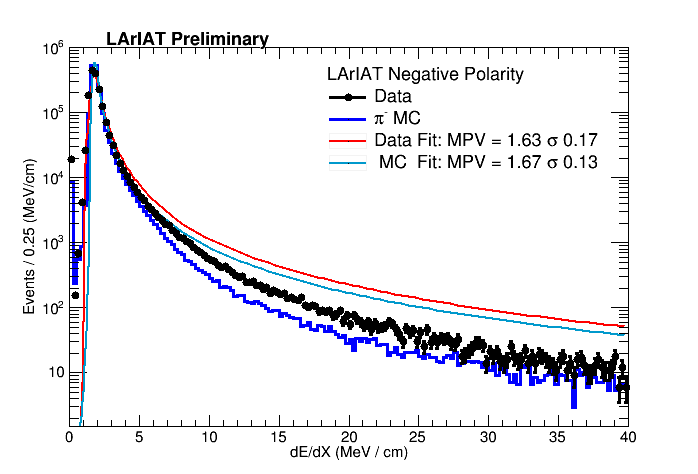
\includegraphics[width=0.48\textwidth]{Studies/Figures/dEdX_Fit_v2.png}
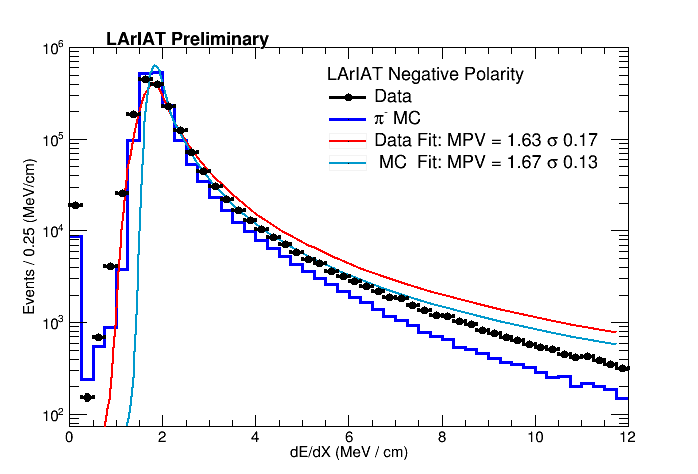
\includegraphics[width=0.48\textwidth]{Studies/Figures/dEdX_Fit_v3.png}
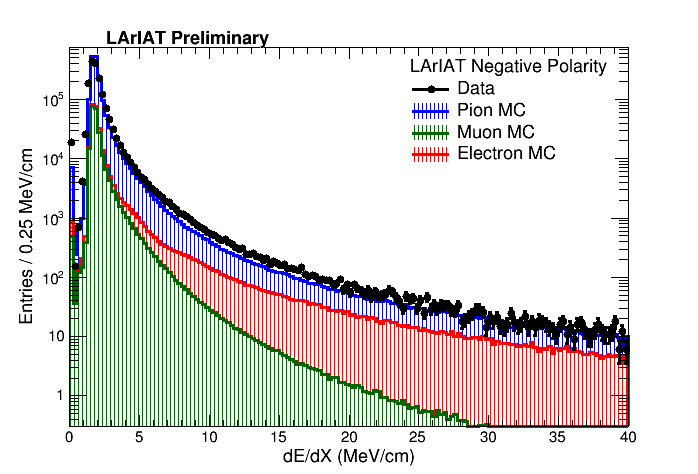
\includegraphics[width=0.48\textwidth]{Studies/Figures/dEdX_stacked_v2.png}
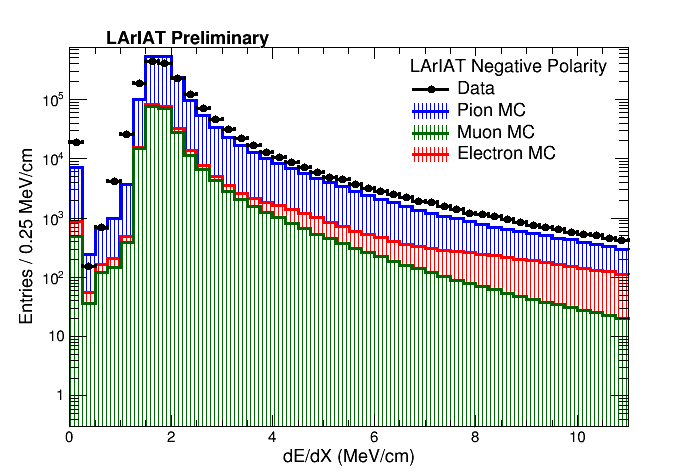
\includegraphics[width=0.48\textwidth]{Studies/Figures/dEdX_stacked_v3.png}
\caption[]{ dE/dX for 60Amp data and MC shown in log scale  } \label{fig:dEdXLogScale}
\end{figure}

Plotting scripts can be found here on lariatgpvm \begin{verbatim}
/lariat/app/users/jasaadi/v06_34_01_PionWeek/PlottingScripts
\end{verbatim} and the samples were put here \begin{verbatim}
/lariat/data/users/elenag/theFinalPions/TPCDATA

/lariat/data/users/elenag/theFinalPions/TPC_MC/
\end{verbatim}

%%%%%%%%%%%%%%%%%%%%%%%%%%%%%%%%%%%%%%%%%%%%%%%
\subsection{Energy Deposited}
%%%%%%%%%%%%%%%%%%%%%%%%%%%%%%%%%%%%%%%%%%%%%%%
The initial energy the particle has as it enters the TPC is given by

\begin{equation}
KE_{Initial} = \sqrt{P_{WCtrk}^2 + m_{\pi}^2} - m_{\pi}^2 - E_{Loss}
\end{equation}

and the uncertainty of the initial energy $\delta KE_{Initial}$ is given by
\begin{equation}
\delta KE_{Initial} = \sqrt{\delta P_{WCtrk}^2 + \delta E_{Loss}^2}
\end{equation}

If we assume the uncertainty is 2\% as the Minerva experiment had, and our uncertainty on the energy loss upstream is 7~MeV, then the total uncertainty on the initial kinetic energy for a typical 500~MeV pion is $\sim 12$~MeV.

% 17/25 data 24/32 MeV for data with an uncertainty of 7 MeV


Now the energy for $j^{th}$ slab of the incident histogram is given by
\begin{equation}
KE^{Incident}_{j} = KE_{Inital} - (\sum_{i<j} dE/dX_{i} \times Pitch_i)
\end{equation}
where $i$ is given by the slab you are at, $dE/dX_{i}$ is the energy deposited at that slab, and $Pitch_i$ is the pitch for that point. 

Thus we can talk about the energy at the $j^{th}$ slab as 

\begin{equation}
E_{j}^{slab} = (\sum_{i<j} dE/dX_{i} \times Pitch_i)
\end{equation}

The systematic uncertainty of $E_{j}^{slab}$ is given by the difference between this quantity in data and MC, and the uncertainty on $E_{j}^{slab}$ is given by the width of the Landau fit to the data. These are shown in Figure \ref{fig:EnergyDeposited}

\begin{figure}[htb]
\centering
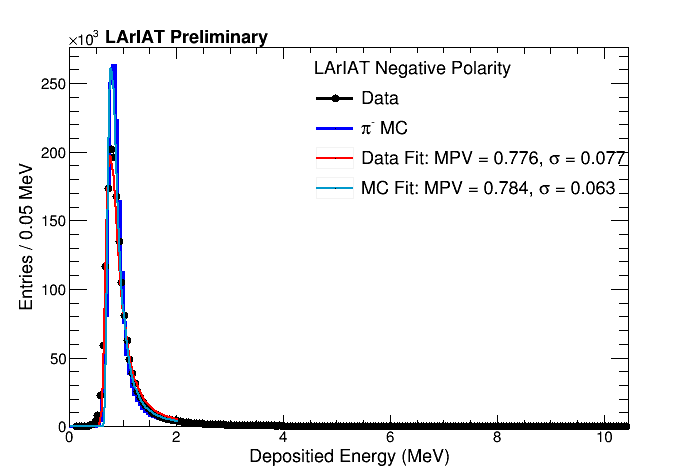
\includegraphics[width=0.48\textwidth]{Studies/Figures/DepEnergy_Fit_v1.png}
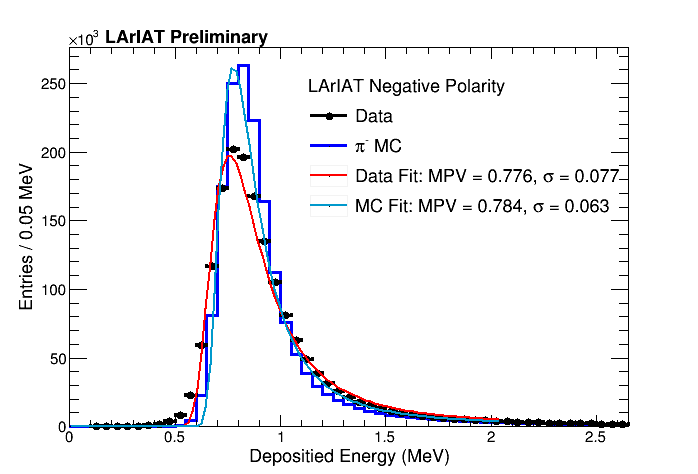
\includegraphics[width=0.48\textwidth]{Studies/Figures/DepEnergy_Fit_v4.png}
\caption[]{ Energy Deposited in Pion MC and 60A data.  } \label{fig:EnergyDeposited}
\end{figure}

The difference between the MPV of data and MC is 1.0\% (0.0784 - 0.0776 / 0.0784) and thus the systematic uncertainty you would assign to the energy in the incident kinetic energy would be for all 240 slices (assuming you have 240 slices at 0.4 mm pitch) and thus is 

\begin{equation}
\delta E^{Slab}_{j} = (0.0784 - 0.0776) \times 240 = 0.008 MeV \times 240 = 1.92 MeV 
\end{equation}

So the uncertainty on the incident kinetic energy is given by

\begin{equation}
\delta KE^{Incident} = \sqrt{ (\delta KE_{Initial})^2 + (\delta E^{Slab}_{j})^2} = \sqrt{(12 MeV)^2 + (2 MeV)^2} = 12.1 MeV
\end{equation}

Figure \ref{fig:EnergyDepositedStacked} shows the stacked version of the Energy Deposited plots with the backgrounds stacked. The backgrounds are given in the ratio of 68.8\% pion, 4.6\% muon, and 26.6\% electron. Once they are taken in these ratios, the sum of the MC is normalized to the sum of the data.

\begin{figure}[htb]
\centering
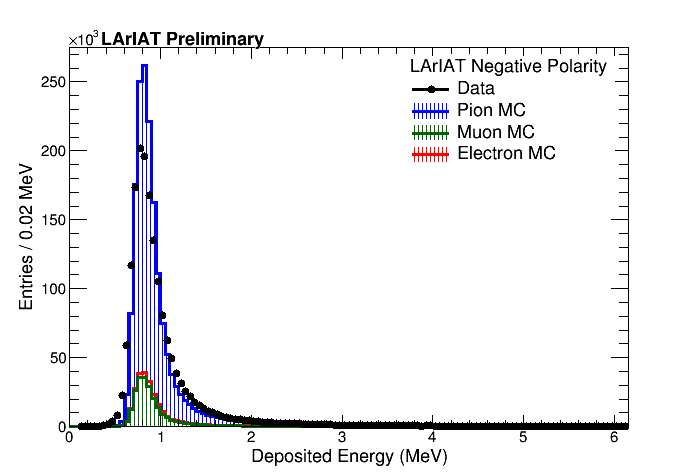
\includegraphics[width=0.48\textwidth]{Studies/Figures/DepEnergy_Stacked_v1.png}
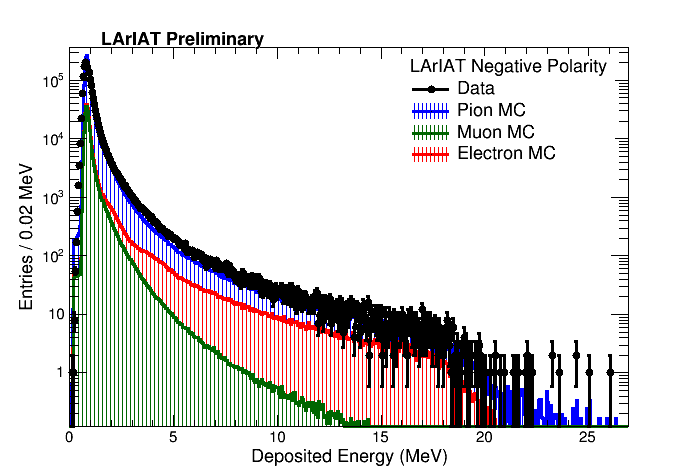
\includegraphics[width=0.48\textwidth]{Studies/Figures/DepEnergy_Stacked_v3.png}
\caption[]{ Energy Deposited with all the MC and 60A data.  } \label{fig:EnergyDepositedStacked}
\end{figure}

The energy at the interacting point is given by
\begin{equation}
KE_{Interaction} = \sqrt{P_{WCtrk}^2 + m_{\pi}^2} - E_{Loss} - (\Sigma dE/dX_{i} \times Pitch)
\end{equation}

and has the exact same uncertainty as the incident kinetic energy plot. Thus these estimates can be applied to getting the uncertainty on the energy of the reconstructed cross-section.


\section{Tracking Studies}

\section{Efficiency Correction}



%%%%%%%%%%%%%%%%%%%%%%%%%%%%%%%%%%%%%%%%%%%%%%%%%%%%%%%%
\begin{comment}
Assuming a beam of pure pions gets to the TPC, let us explicit some of the variables in the kinetic energy equation \ref{eq:KEj}  to point out the important quantities in the uncertainty budget,

\begin{align}
 E_{j}^{kin} &=  E_{Beam}^{kin}  - E_{loss} - \sum_{i < j} \frac {dE_i}{dx_i}*dx_i\\
                  &=  \sqrt{p^2_{Beam} - m^2_{Beam}} - m_{Beam} - E_{loss} - \sum_{i < j} \frac {dE_i}{dx_i}*dx_i.
\end{align}

\subsection{Uncertainty on $E_{Beam}^{kin}$}
Let us start by discussing the uncertainty on $E_{Beam}^{kin}$. Since we are assuming a beam of pions, the uncertainty on the value of mass of the pion ($m_{Beam}$) as given by the pdg is irrelevant compared to the momentum uncertainties, thus $\delta E_{Beam}^{kin} = \delta p_{Beam}^{kin}$. 
We estimate the momentum uncertainty as follows.

\textcolor{blue}{  
We estimate the uncertainty on a 4-point track. In case of 3-points track, we add an additional 2\% coming from Greg's study. 
Uncertainty on a 4-point track:
\begin{itemize}
\item[-]  Alignment surveys. 1mm misalignment translates to 3\% in overall
\item[-] Doug study dp/p = ~2\% based on field map (docdb 1710)
\item[-] Minerva test beam paper
\end{itemize}
}

\subsection{Systematics on $E_{loss}$}




\textbf{Systematics}
Discrepancies between the real TPC geometry and the simulated geometry can lead to a systematic in the $E_{loss}$ calculation. In particular, we found a difference in the depth of the un-instrumented argon upstream to the TPC front face, the MC geometry reporting $~\sim 3.3$ cm more un-instrumented argon than the TPC survey. For a pion MIP, this depth corresponds to 7.4 MeV which we account for as a double sided systematic in the determination of the pion kinetic energy.

\subsection{Uncertainty on dE/dx and pitch}
We obtain the uncertainty on dE/dx and track pitch by comparing the dE/dx and pitch distributions in data and MC.
\textcolor{blue}{ Currently, MPV MC = 1.70 and MPV DATA = 1.72 MeV/cm (~3\% higher).
TO DO HERE: calculate Argon density from mid-RTD temperature. Compare this  density with MC Argon density. 
Density change  affects dE/dx (in MeV/cm!). Try changing MC density up to ``real one" and see if dEdX agrees between DATA and MC}


\subsection{Uncertainty on track end, aka efficiency correction}
From the MC, we obtain an efficiency correction on the interacting and incident distributions separately. This is done by comparing the MC reconstructed with the true MC deposition on an event by event basis.
This correction is applied bin by bin on the data interacting and incident distributions.
The better our tracking, the smaller this efficiency correction will be. So, step number one is improving the tracking.
\textcolor{blue}{Need to talk to Bruce about this.}
\textcolor{blue}{ I don't understand the angle cut that Dave Schmitz and Jon Paley were so vocal about.}

Now, the key question remains: does the tracking behave in the same way in data and MC? 
We can compare some key plots between reconstructed data and MC which gives us confidence this is true: the track pitch, the tracks straightness and the goodness of fit in data and MC. \textcolor{blue}{ Does such a variable as ``goodness of fit" exists in the tracking? We should ask Bruce.}
\end{comment}
